%
\begin{isabellebody}%
\setisabellecontext{Introduction}%
%
\isadelimtheory
%
\endisadelimtheory
%
\isatagtheory
%
\endisatagtheory
{\isafoldtheory}%
%
\isadelimtheory
%
\endisadelimtheory
%
\isadelimdocument
%
\endisadelimdocument
%
\isatagdocument
%
\isamarkupchapter{Introduction%
}
\isamarkuptrue%
%
\endisatagdocument
{\isafolddocument}%
%
\isadelimdocument
%
\endisadelimdocument
%
\begin{isamarkuptext}%
In this thesis, I show the correspondence between various equivalences popular in the reactive
systems community and coordinates of a formula price function, as introduced by Bisping in \cite{bisping2023process}. I formalized the concepts and proofs discussed in this thesis in the interactive proof assistant Isabelle.

\textit{Reactive systems} are computing systems that continuously interact with their environment, reacting to external stimuli and producing outputs accordingly \cite{harel85}.
At a high level of abstraction, these systems can be seen as collections of interacting processes, where each process represents a state or configuration of the system. 
Labeled Transition Systems (LTS) \cite{keller76} provide a formal framework for modeling and analyzing the behavior of reactive systems. Roughly, an LTS is a labeled directed graph, whose nodes denote the processes
and whose edges correspond to transitions between those processes (or states).

Verification of these systems involves proving statements regarding the behavior of such a system model. Often, verification tasks aim to show that a system's observed behavior aligns with its intended behavior.
That requires a criterion of what constitutes similar behavior on LTS, commonly referred to as the \textit{semantics of equality} of processes. Depending on the requirements of a particular user, many different such criterions have been defined.
For a subset of processes, namely the class of concrete sequential processes, \cite{GLABBEEK20013} classified many such semantics. 
\textit{Sequential} means that the processes can only perform one action at a time. \textit{Concrete} processes are processes in which no internal actions occur, meaning that it exclusively captures the system's interactions with its environment.
In such LTS, every transition represents an observable event or action between the system and its environment.
The classification in \cite{GLABBEEK20013} involved partially ordering many of these semantics by the relation 'makes strictly more identifications on processes than'. The resulting lattice is
known as the (infinitary) linear-time--branching-time spectrum \footnote{On Infinity?} 
\footnote{Linear time describes identification via the order of events, while branching time captures the branching possibilities in system executions.}.
One way to characterize the behavior of LTS is through the use of modal logics. Formulas of a logic can be seen as describing certain properties of states within an LTS. A commonly used modal logic is Hennessy-Milner logic (HML) \cite{hm85}. 
Equivalence in terms of HML is determined by whether processes satisfy the same set of formulas. The linear-time--branching-time spectrum can be recharted in terms of the subset relation between these modal-logical characterizations.%
\end{isamarkuptext}\isamarkuptrue%
%
\begin{isamarkuptext}%
In the context of this spectrum, demonstrating that a system model's observed behavior aligns with the behavior of a model of the specification can be done by 
finding the finest notions of behavioral equivalence that equate them. Special bisimulation games and algorithms capable of answering equivalence questions 
by performing a 'spectroscopy' of the differences between two processes have been developed \cite{bisping2022deciding}\cite{bisping2023process}.
These approaches rechart the linear-time--branching-time spectrum using an expressiveness function that assigns a \textit{formula price} to every formula. 
This price is supposed to capture the expressive capabilities of a particular formula. However, to be sure that these characterizations really capture the desired equivalences one has to perform the proofs.%
\end{isamarkuptext}\isamarkuptrue%
%
\begin{isamarkuptext}%
\begin{figure}[htbp]
    \centering
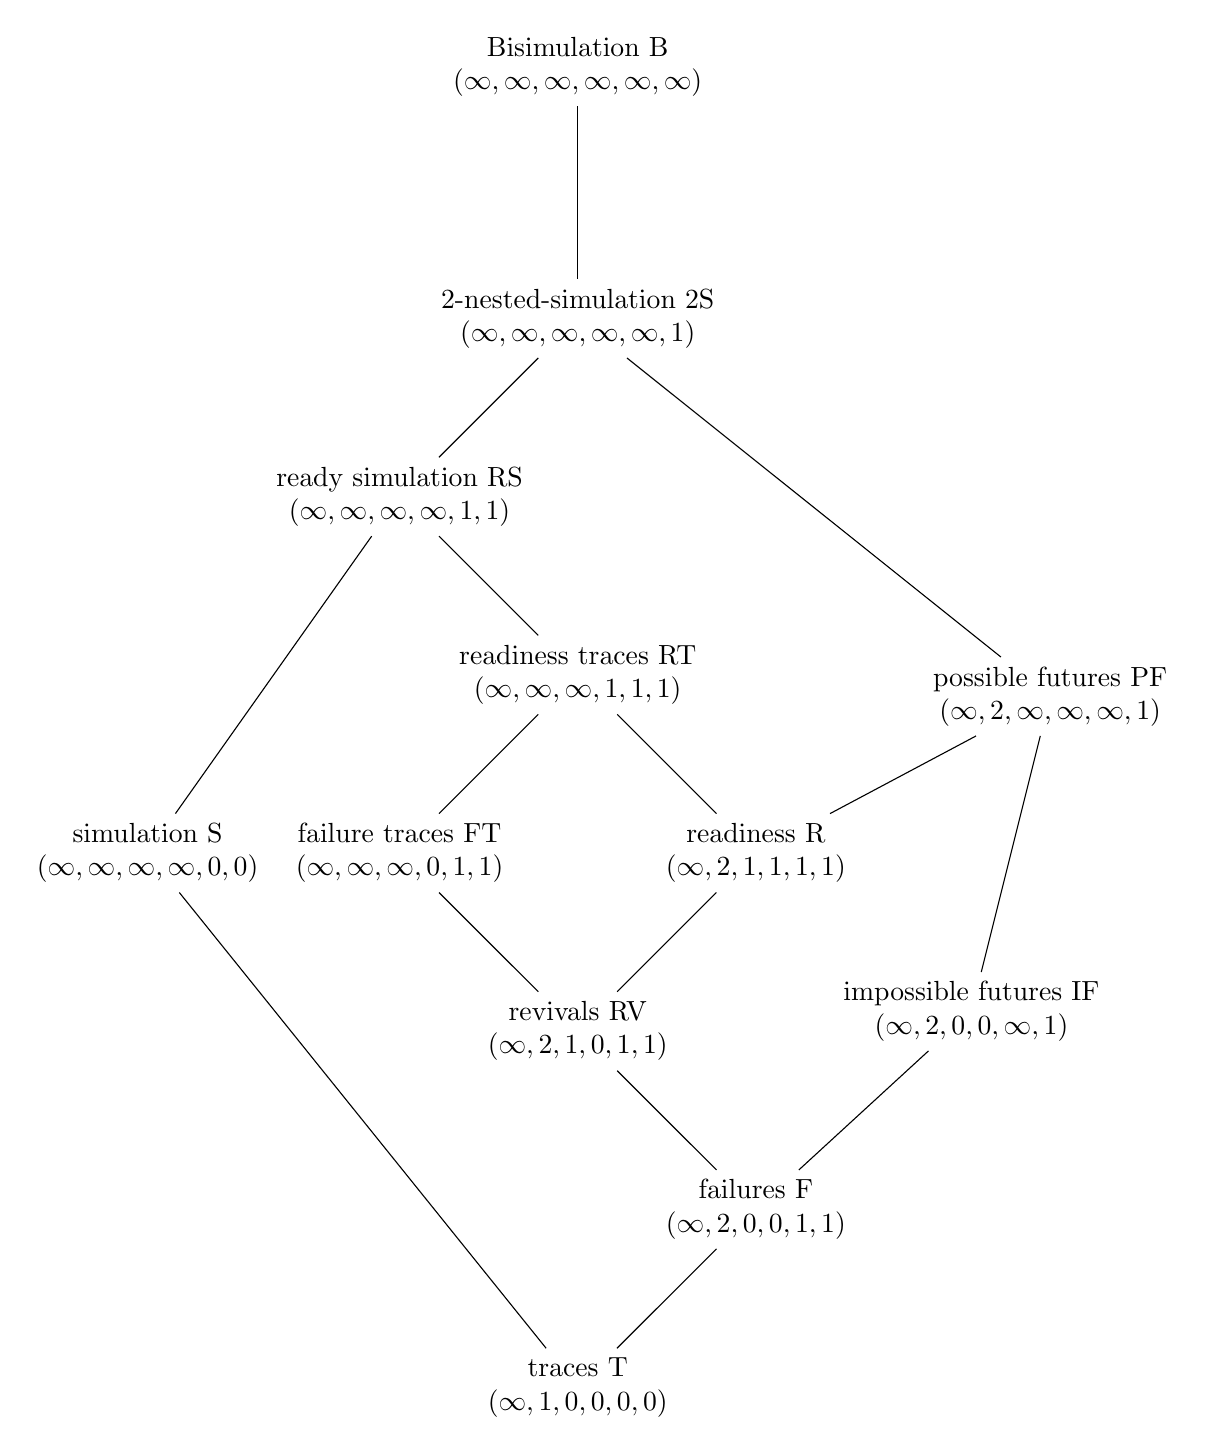
\begin{tikzpicture}[auto,node distance=3.2cm] % Adjusted node distance
  \node[align=center] (B) {Bisimulation B\\$(\infty, \infty, \infty, \infty, \infty, \infty)$};
  \node[align=center, below of=B] (2S) {2-nested-simulation 2S\\$(\infty, \infty, \infty, \infty, \infty, 1)$};
  \node[align=center, below left of=2S] (RS) {ready simulation RS\\$(\infty, \infty, \infty, \infty, 1, 1)$};
  \node[align=center, below right of=RS] (RT) {readiness traces RT\\$(\infty, \infty, \infty, 1, 1, 1)$};
  \node[align=center] (PF) at (6,-8) {possible futures PF\\$(\infty, 2, \infty, \infty, \infty, 1)$};
  \node[align=center, below left of=RT] (FT) {failure traces FT\\$(\infty, \infty, \infty, 0, 1, 1)$};
  \node[align=center, left of=FT] (S) {simulation S\\$(\infty, \infty, \infty, \infty, 0, 0)$};
  \node[align=center, below right of=RT] (R) {readiness R\\$(\infty, 2, 1, 1, 1, 1)$};
  \node[align=center, below left of=R] (RV) {revivals RV\\$(\infty, 2, 1, 0, 1, 1)$};
  \node[align=center] (IF) at (5,-12) {impossible futures IF\\$(\infty, 2, 0, 0, \infty, 1)$};
  \node[align=center, below right of=RV] (F) {failures F\\$(\infty, 2, 0, 0, 1, 1)$};
  \node[align=center, below left of=F] (T) {traces T\\$(\infty, 1, 0, 0, 0, 0)$};

  
  \draw[-] (B) -- node[above] {} (2S);
  \draw[-] (2S) -- node[left] {} (RS);
  \draw[-] (2S) -- node[right] {} (PF);
  \draw[-] (RS) -- node[left] {} (S);
  \draw[-] (RS) -- node[left] {} (RT);
  \draw[-] (PF) -- node[left] {} (IF);
  \draw[-] (RT) -- node[left] {} (FT);
  \draw[-] (RT) -- node[left] {} (R);
  \draw[-] (FT) -- node[left] {} (RV);
  \draw[-] (R) -- node[left] {} (RV);
  \draw[-] (R) -- node[left] {} (PF);
  \draw[-] (RV) -- node[left] {} (F);
  \draw[-] (IF) -- node[left] {} (F);
  \draw[-] (F) -- node[left] {} (T);
  \draw[-] (S) -- node[left] {} (T);
\end{tikzpicture}
\caption{TEEEEEEEEEEEEEEEEEEST}
    \label{fig:your_label}
\end{figure}%
\end{isamarkuptext}\isamarkuptrue%
%
\isadelimdocument
%
\endisadelimdocument
%
\isatagdocument
%
\isamarkupsubsubsection{Contributions%
}
\isamarkuptrue%
%
\endisatagdocument
{\isafolddocument}%
%
\isadelimdocument
%
\endisadelimdocument
%
\begin{isamarkuptext}%
This thesis provides a machine-checkable proof that the price bounds of the expressiveness function $\textsf{expr}$ of \cite{bisping2023process} correspond to the modal-logical characterizations of named equivalences. 
More precisely, we consider a formula $\varphi$ to be in an observation language $\mathcal{O}_X$ iff its price is within the given price bound.
For every expressiveness price bound $e_X$, we derive the sublanguage of Hennessy--Miler logic $\mathcal{O}_X$ and show that a formula $\varphi$ is in $\mathcal{O}_X$ precisely if its price \isa{expr{\isacharparenleft}{\kern0pt}{\isasymphi}{\isacharparenright}{\kern0pt}} is less than or equal to $e_X$.
Then we show that $\mathcal{O}_X$ has exactly the same distinguishing power as the modal-logical characterization of that equivalence.
In (ref Foundations (chapter 2)) we discuss and introduce formal definitions of LTSs, Hennessy-Milner logic and the expressiveness function $\textsf{expr}$. In (ref The Correspondances?! name!) we provide modal-logical definitions and perform
the proofs for the standard notions of equivalence, i.e. the equivalences of (ref Figure 1). Namely for trace-, failures-, failure-trace-, readiness-, ready-trace-, revivals-, possible-futures-, impossible-futures-, simulation-, ready-simulation-, 2-nested-simulation- and bisimulation semantics.
All the main concepts and proofs have been formalized and conducted using the interactive proof assistant Isabelle. More information on Isabelle can be found in (appendix?).
We tried to present Isabelle implementations directly after their corresponding mathematical definitions.
The mathematical definitions are marked as 'definitions' and presented in standard text format. Their corresponding Isabelle implementations
are presented right after, distinguished by their \isa{monospaced\ font} and \textcolor{RoyalBlue}{colored} \textcolor{ForestGreen}{syntax} \textcolor{Cerulean}{highlighting}.
However, for readability purposes, a majority of the Isabelle proofs are hidden and replaced by \isa{{\isasymproof}} and some lemmas excluded. The whole Isabelle code and a web version of this thesis can be found on Github\footnote{\textcolor{red}{Link!!!}}.%
\end{isamarkuptext}\isamarkuptrue%
%
\isadelimtheory
%
\endisadelimtheory
%
\isatagtheory
%
\endisatagtheory
{\isafoldtheory}%
%
\isadelimtheory
%
\endisadelimtheory
%
\end{isabellebody}%
\endinput
%:%file=~/Documents/Isabelle_HOL/Introduction.thy%:%
%:%24=8%:%
%:%36=9%:%
%:%37=10%:%
%:%38=11%:%
%:%39=12%:%
%:%40=13%:%
%:%41=14%:%
%:%42=15%:%
%:%43=16%:%
%:%44=17%:%
%:%45=18%:%
%:%46=19%:%
%:%47=20%:%
%:%48=21%:%
%:%49=22%:%
%:%50=23%:%
%:%51=24%:%
%:%52=25%:%
%:%53=26%:%
%:%57=38%:%
%:%58=39%:%
%:%59=40%:%
%:%60=41%:%
%:%61=42%:%
%:%65=46%:%
%:%66=47%:%
%:%67=48%:%
%:%68=49%:%
%:%69=50%:%
%:%70=51%:%
%:%71=52%:%
%:%72=53%:%
%:%73=54%:%
%:%74=55%:%
%:%75=56%:%
%:%76=57%:%
%:%77=58%:%
%:%78=59%:%
%:%79=60%:%
%:%80=61%:%
%:%81=62%:%
%:%82=63%:%
%:%83=64%:%
%:%84=65%:%
%:%85=66%:%
%:%86=67%:%
%:%87=68%:%
%:%88=69%:%
%:%89=70%:%
%:%90=71%:%
%:%91=72%:%
%:%92=73%:%
%:%93=74%:%
%:%94=75%:%
%:%95=76%:%
%:%96=77%:%
%:%97=78%:%
%:%98=79%:%
%:%99=80%:%
%:%100=81%:%
%:%109=83%:%
%:%121=85%:%
%:%122=86%:%
%:%123=87%:%
%:%124=88%:%
%:%125=89%:%
%:%126=90%:%
%:%127=91%:%
%:%128=92%:%
%:%129=93%:%
%:%130=94%:%
%:%131=95%:%
